%%%%%%%%%%%%%%%%%%%%%%%%%%%%%%%%% Článok %%%%%%%%%%%%%%%%%%%%%%%%%%%%%%%%%%%%%%
\documentclass[10pt,twoside,slovak,a4paper]{article}
%%%%%%%%%%%%%%%%%%%%%%%%%%%%%%%%%%%%%%%%%%%%%%%%%%%%%%%%%%%%%%%%%%%%%%%%%%%%%%%

%%%%%%%%%%%%%%%%%%%%%%%%%%%%%%%%% Balíky %%%%%%%%%%%%%%%%%%%%%%%%%%%%%%%%%%%%%%
\usepackage[slovak]{babel}
\usepackage[IL2]{fontenc}
\usepackage[utf8]{inputenc}
\usepackage{graphicx}
\usepackage{url}
\usepackage{hyperref} % odkazy v texte budú aktívne (pri niektorých triedach dokumentov spôsobuje posun textu)
\usepackage{float}
\usepackage{cite}
\usepackage{times}
\usepackage{lmodern}
\usepackage{geometry}
\usepackage{amssymb}
\usepackage{amsmath}
\usepackage{cancel}
\usepackage{amsthm}
\usepackage{empheq}
\usepackage{mdframed}
\usepackage{booktabs}
\usepackage{lipsum}
\usepackage{color}
\usepackage{psfrag}
\usepackage{pgfplots}
\usepackage{bm}
%%%%%%%%%%%%%%%%%%%%%%%%%%%%%%%%%%%%%%%%%%%%%%%%%%%%%%%%%%%%%%%%%%%%%%%%%%%%%%%

%%%%%%%%%%%%%%%%%%%%%%%%%%%%%%% Nastavenia Strany %%%%%%%%%%%%%%%%%%%%%%%%%%%%%
\usepgfplotslibrary{colorbrewer}
\pgfplotsset{width=8cm,compat=1.9}
\pagestyle{headings}
\raggedbottom
%%%%%%%%%%%%%%%%%%%%%%%%%%%%%%%%%%%%%%%%%%%%%%%%%%%%%%%%%%%%%%%%%%%%%%%%%%%%%%%

%? Okolo 5 stran
%TODO Fixnut odsadenie textu
%TODO Opravit alebo odstranit cisla v zahlavy stran
%TODO Pridať obsah článku
%TODO Dopísať sekcie

%%%%%%%%%%%%%%%%%%%%%%%%%%%%%%%%%%%%%% Autor %%%%%%%%%%%%%%%%%%%%%%%%%%%%%%%%%%
\title{Kultúrny model pre správanie nehrateľných postav v počítačových hrách\thanks{Semestrálny projekt v predmete Metódy inžinierskej práce, ak\@. rok 2021/22, vedenie cvičení: Ing. Fedor Lehocki, PhD.}}
\author{Martin Szabo\\[2pt]
	{\small Slovenská technická univerzita v Bratislave}\\
	{\small Fakulta informatiky a informačných technológií}\\
	{\small \texttt{xszabom5@stuba.sk}}
	}
\date{\small 6.\ november 2021}
%%%%%%%%%%%%%%%%%%%%%%%%%%%%%%%%%%%%%%%%%%%%%%%%%%%%%%%%%%%%%%%%%%%%%%%%%%%%%%%

%%%%%%%%%%%%%%%%%%%%%%%%%%%%%%%%%%%%% Abstrakt %%%%%%%%%%%%%%%%%%%%%%%%%%%%%%%%
\begin{document}

\maketitle
\begin{abstract}

Počítačové hry sa často snažia čo najbližšie priblížiť realite. Veľa hier sa snaží priblížiť realite práve tým že 
majú realistickú fyziku a grafiku. Ale málo hier sa zaoberá tým ako sa nehrateľné postavy tzv. `NPC' z anglického
`Non-playable character' správajú v hernom svete. Aby sme sa priblížili k realite čo najviac je dôležité aby postavy
dokázali prejavovať emócie, mať osobnostné črty a samozrejme správať sa sociálne aby sme získali dojem že tá postava
myslí a žije aj keď je to len pár pixelov v počítačovej hre. Model ktorým sa tento článok zaoberá ponúka lepšie
možnosti ako modelovať realistickejší vzor správania.

\end{abstract}
%%%%%%%%%%%%%%%%%%%%%%%%%%%%%%%%%%%%%%%%%%%%%%%%%%%%%%%%%%%%%%%%%%%%%%%%%%%%%%%


%%%%%%%%%%%%%%%%%%%%%%%%%%%%%%%%%%%%% Úvod %%%%%%%%%%%%%%%%%%%%%%%%%%%%%%%%%%%%
\section{Úvod}

Herný priemysel je jeden z najpopulárnejších a najrýchlejšie rastúcich priemyslov.
Tisíce eur sa investujú do rôznych technológií na vývoj hier a panuje tam veľká konkurencia
medzi jednotlivými vývojárskymi firmami. Každý sa snaží mať tú najlepšiu a najpopulárnejšiu
hru v celom priemysle. Tento priemysel je zaplavený rôznymi hrami ktoré pokiaľ chcú zaujať hráčov
tak musia robiť niečo unikátnejšie než ich konkurencia. V tomto článku sa budeme zaoberať témou
kultúrneho modelu nehrateľných postav ktorá je veľakrát podceňovaná. Namodelovanie správnej kultúry
nehrateľných postav hráčom ponúka hlbšie emočné spojenie s postavami v príbehu a pomáha hráčovi
vžiť sa do herného sveta. Existujú hry ktoré simulovali rôzne kultúry ale žiadne to nerobili do takej 
miery ako to vidíme v reálnom svete. Postava ktorá bude namodelovaná cez model predstavený v 
tomto článku bude schopná nie len patriť pod nejakú kultúru ale aj správať sa adekvátne v rámci
jej kultúrneho modelu. Bude reagovať na zlé a dobré podnety od hráča ale aj od iných nehrateľných 
postáv a bude môcť prejavovať široké spektrum emócií rovnako ako to je aj v realite u ľudí. Taktiež bude 
môcť usúdiť na základe správania hráča a iných nehrateľných postav okolo nej jej vzťah k nim. Tento model
sa bude usilovať o simuláciu reálnej mysle človeka a následne bude z neho vyplývať správanie nehrateľných
postav v hernom svete.

%%%%%%%%%%%%%%%%%%%%%%%%%%%%%%%%%%%%%%%%%%%%%%%%%%%%%%%%%%%%%%%%%%%%%%%%%%%%%%%

%%%%%%%%%%%%%%%%%%%%%%%%%%% Základne modely a pojmy %%%%%%%%%%%%%%%%%%%%%%%%%%%
\section{Základne modely a pojmy}\label{zaklad}

Základne modely z ktorých bude tento model vychádzať primárne z Plutchikoveho kolesa emócií
(Obr.~\ref{fig:EWheel}). Emócie sú stavy ktoré sa odohrávajú v našom nervovom systéme. Sú to chemické
procesy ktoré súvisia s našim správaním, pocitmi a myšlienkami. Existuje veľa teórií ktoré sa snažia
vysvetliť ako emócie súvisia s osobnosťou. Pre tento model najlepšie funguje práve teória Jamesa Langeho.
Jeho teória naznačuje že emócie sú výsledkom fyziologických reakcií na podnety a udalosti. Taktiež existuje
teória Paula Ekmana ktorý definuje emócie ako diskrétne, merateľné a z psychologického hľadiska
rozdielne, definoval 6 základných emócií:

\begin{enumerate}
	\item Hnev
	\item Znechutenie
	\item Strach
	\item Šťastie
	\item Smútok
	\item Prekvapenie
\end{enumerate}

Robert Plutchik rozšíril teóriu Ekmana a vytvoril tzv. Koleso Emócií. V tejto teórií je 8
emočných sektorov s troma úrovňami intenzity pre každú emóciu. Napríklad žltá os má najnižšie
emóciu pokoj. V strede má radosť a najvyššie má extázu Jednotlivé emócie sa môžu v tomto modeli
aj miešať. Miešanie emócií majú rôzne úrovne:

\begin{itemize}
	\item Primárne (často viditeľné)
	\item Sekundárne (občas viditeľné)
	\item Terciárna (zriedka viditeľné)
	\item Opačné (neviditeľné)
\end{itemize}

Dobrý príkladom kombinácie emócií na primárnej úrovni sú radosť a dôvera.
Kombináciou týchto dvoch emócií dostaneme lásku. Príklad sekundárnej kombinácie
emócií je radosť a strach z ktorých nám vznikne vzrušenie. Terciárna kombinácia
emócií môže byť napríklad radosť a prekvapenie z ktorých nám vyplýva potešenie.

\begin{figure}[H]
		\centering
		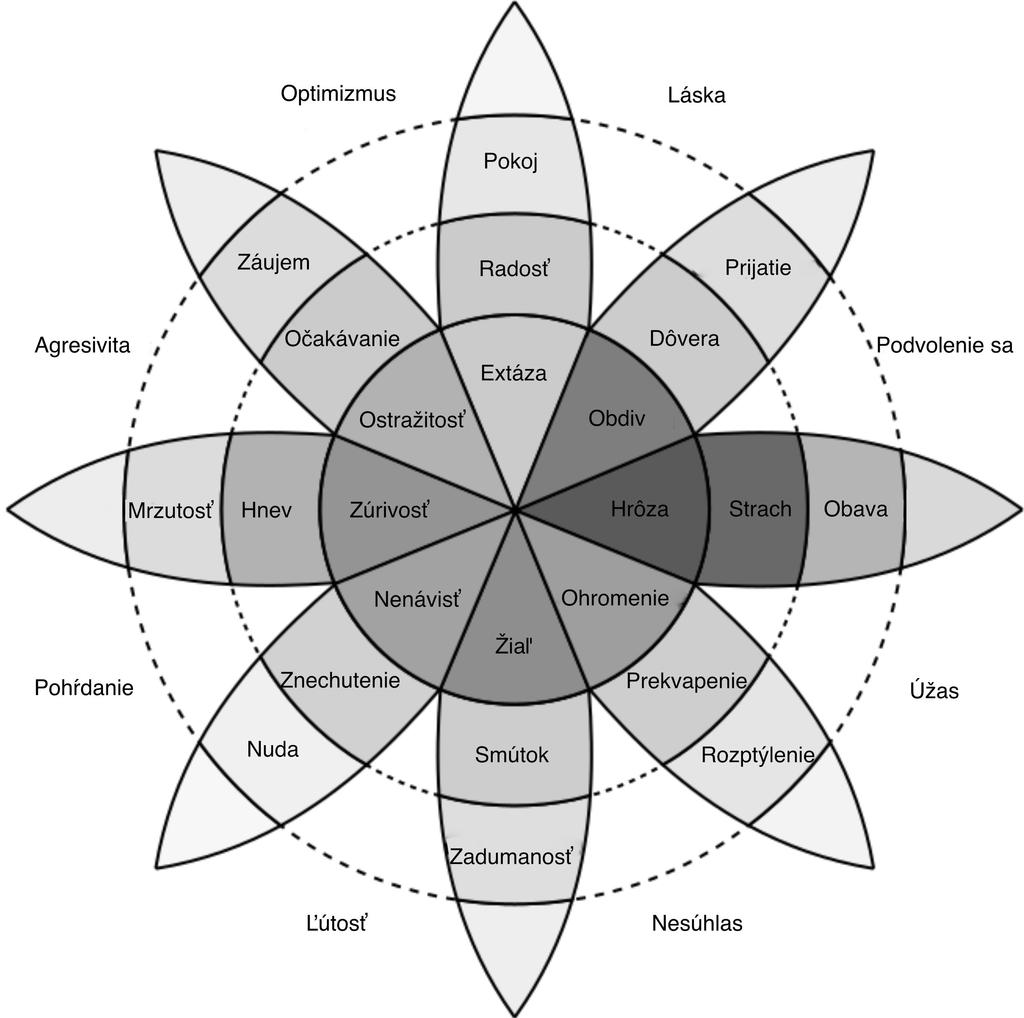
\includegraphics[scale=0.40]{Obrázky/Plutchikove_koleso.jpg}
		\caption{Plutchikové koleso emócií~\cite{emocie}}
		\label{fig:EWheel}
\end{figure}

\pagebreak
%%%%%%%%%%%%%%%%%%%%%%%%%%%%%%%%%%%%%%%%%%%%%%%%%%%%%%%%%%%%%%%%%%%%%%%%%%%%%%%

%%%%%%%%%%%%%%%%%%%%%%%%%%%%%%%%%% Proxemika %%%%%%%%%%%%%%%%%%%%%%%%%%%%%%%%%%
\section{Proxemika}\label{proxemika}

Proxemika je vedna disciplína ktorá sa zaobera tým ako ľudia využívajú priestor v
socialnej komunikácií a aký to má dopad na správanie členov komunikácie. Edward T. Hall,
vyznmaný antropológ ktorý v svojej práci o proxemike ju definoval ako~\cite{proxemics} ``Pozorovania a teórie
ľudi používajúci priesto ako špecializované vypracovanie kultúry''. Proxemika nie je dôležitá
len v komunikácie ale v širom ponímani aj v organizácií priestoru.

\subsection{Ako funguje proxemika}\label{proxemika:funkcnost}

Proxemika~\cite{proxemika} v socialnej komunikácií je osobná zóna, ktorá obklopuje každého človeka. Vieme si ju
predstaviť ako fiktívnu bublinu. Od ľudí ktorý sú nám nesympatickí si držíme inú vzdialenosti ako
od neznámych.Najmenej sa odťahujeme od detí, rodiny, priateľov alebo veľmi blízkych ľudí. Podľa
toho môžeme priestor okolo nás rozdeliť na tieto zóny (Obr.~\ref{fig:proxemics}):

\begin{enumerate}
	\item Intímna zóna (Intimate) - je dotykový kontakt, to znamená, že je typická pre blízky kontakt do 30 cm (napr. matka - dieťa, milenci, blízki priatelia), oznamujeme v nej osobné, prípadne až intímne informácie.
	\item Osobná zóna (Personal) - hranica vzdialenosti 40 - 80 cm pre priateľov, s cudzím človekom 45 - 120 cm (napr. dobrý očný kontakt,  podanie ruky).
	\item Sociálna zóna (Social) - partneri nie sú osobne zaujatí, 120 - 360 cm (narp. obchodné jednanie, služobný kontakt). Je to dobrý kontakt, ale je vhodné zvýšiť hlas.
	\item Verejná zóna (Public) - začína pri 360 a končí približne pri 760 cm (napr. herec, učiteľ na prednáške), vôbec nie je vhodná na osobnú, intímnu komunikáciu, nevidno na ústa ani do očí a je potrebné hovoriť hlasnejšie.
\end{enumerate}

Fungovanie tohto princípu je ovplyvnené aj osobnosťou jednotlivca. Vzdialenosti jednotlivých
zón sú preto vždy v určitom rozsahu. Najviac sme citliví na narušenie intímnej a osobnej zóny
nevhodnými ľuďmi, presne podľa popisu, čo môže vyvolať prekvapivé reakcie.

\begin{figure}[H]
	\centering
	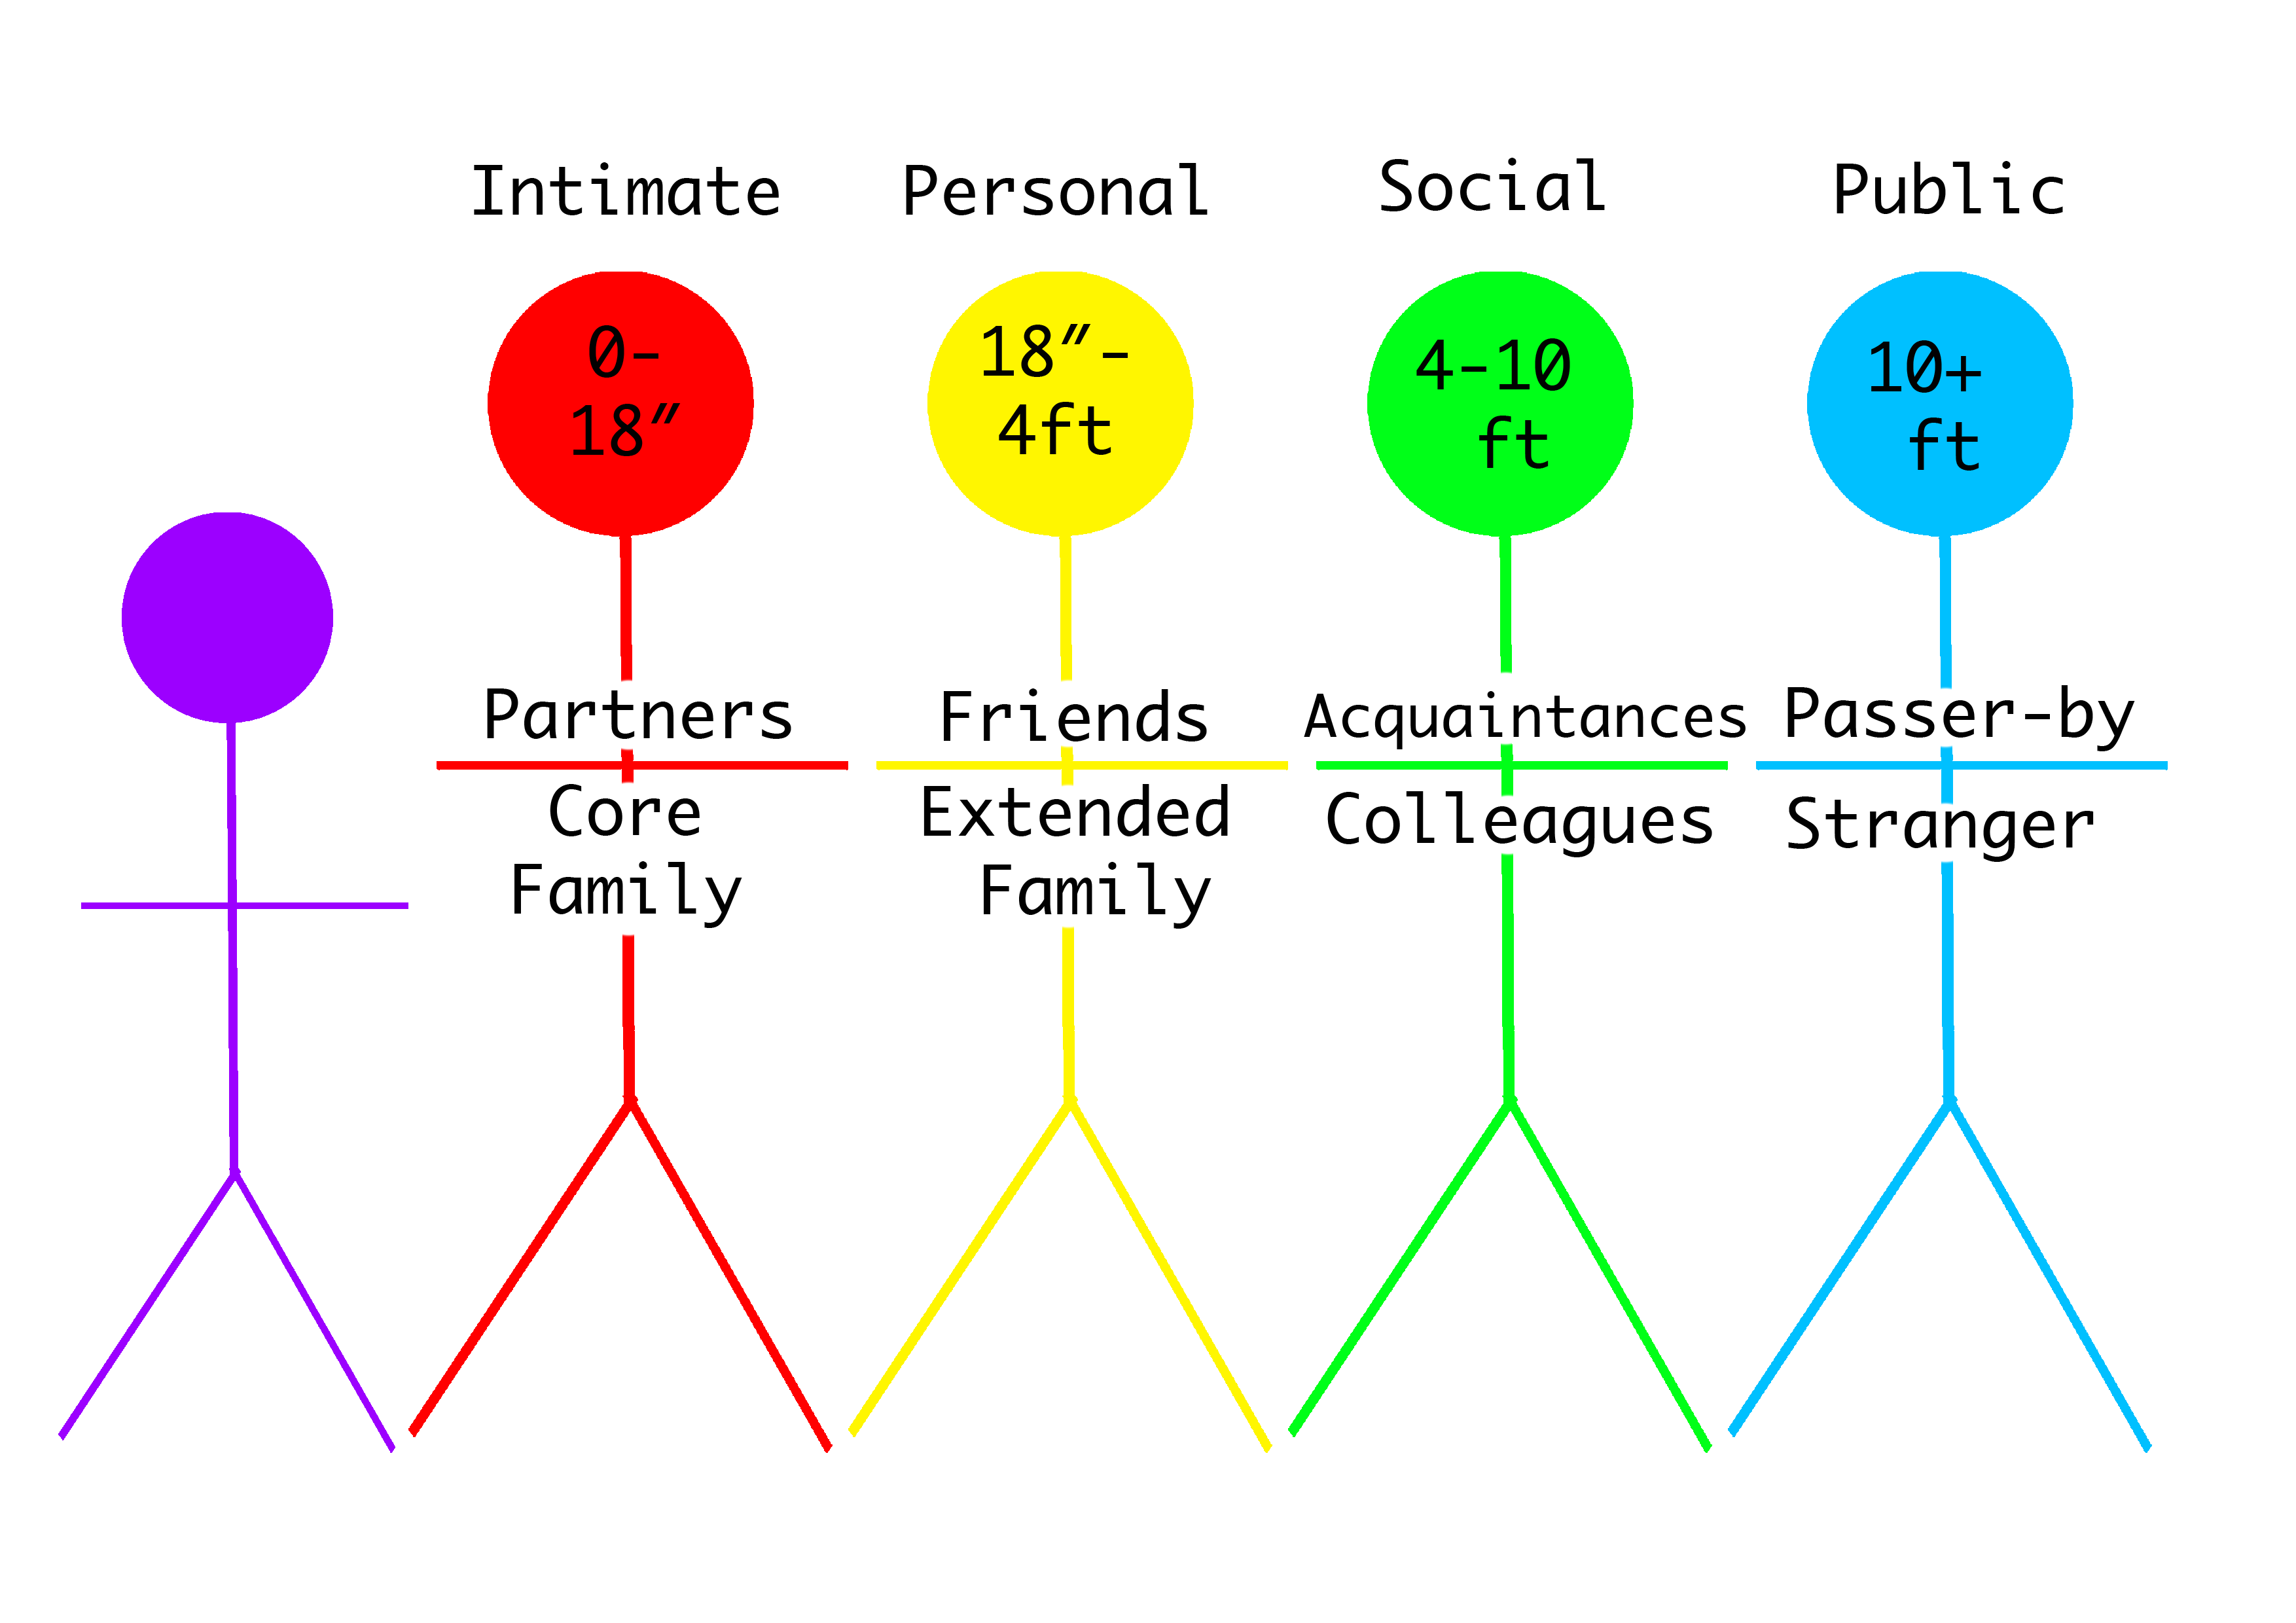
\includegraphics[scale=0.34]{Obrázky/Proxemics.png}
	\caption{Proxemika~\cite{hall1966the} (Osobný priestor)}
	\label{fig:proxemics}
\end{figure}


\subsection{Ako využijeme poznatky z proxemiky v modeli}\label{proxemika:poznatky}

Definíciu Edwarda T. Halla využijeme v tomto modeli lebo proxemika v hrách určuje ako reagujú
ostatné postavy keď sa k ním priblížite do ich osobného priestoru ale aj ako sú mestá v hrách
postavené. Proxemiku ako takú však ale môžeme využiť pri mnohých oblastiach vývoja počítačových
hier.

\pagebreak
%%%%%%%%%%%%%%%%%%%%%%%%%%%%%%%%%%%%%%%%%%%%%%%%%%%%%%%%%%%%%%%%%%%%%%%%%%%%%%%

%%%%%%%%%%%%%%%%%%%%%%%%%%%%%%% Kultúrne dimenzie %%%%%%%%%%%%%%%%%%%%%%%%%%%%%
\section{Kultúrne dimenzie}\label{kultura} 

Kultúrne dimenzie definoval holandský vedec Geert Hofstede ako \cite{hofstede2010cultures}
``Kolektívne programovanie mysle, ktoré odlišuje členov jednej skupiny alebo kategórie ľudí
od ostatných''. Keďže v našom modeli potrebujeme reprezentovať kultúru v hre dimenzie definované
v tejto teórií vieme použiť v našom modeli efektívne. Táto teória ponúka 6 základných kultúrnych
dimenzií (Obr.~\ref{fig:culture}).

\begin{figure}[H]
	\centering
	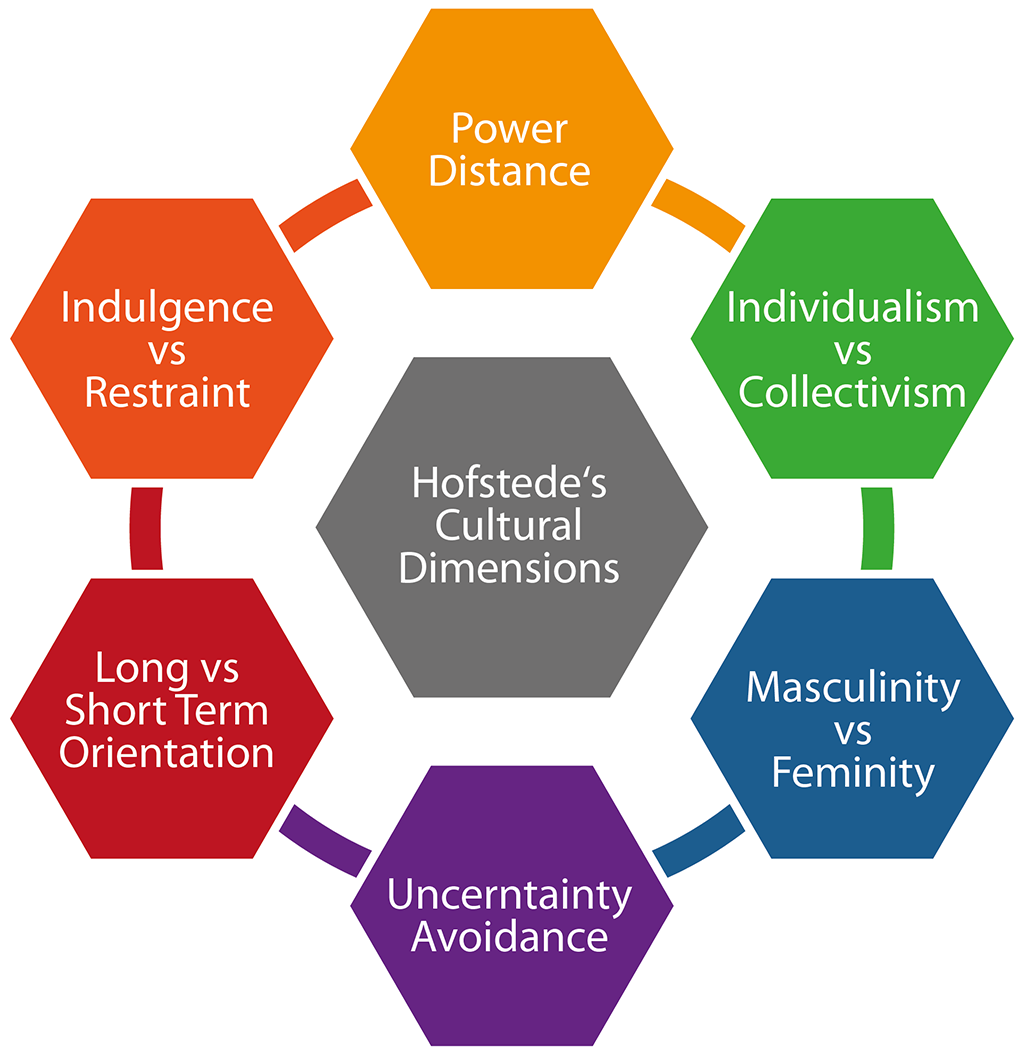
\includegraphics[scale=0.34]{Obrázky/Cultural_dimensions.png}
	\caption{Základné kultúrne dimenzie~\cite{hofstede2010cultures}}
	\label{fig:culture}
\end{figure}

\subsection{Distribúcia moci}\label{kultura:moc}

Distribúcia moci znamená, do akej miery menej mocný členovia inštitúcií a organizácií v
rámci krajiny očakávajú a akceptujú, že moc v krajine je nerovnomerne distribuovaná. Tato
vlastnosť je rozdielna od krajiny v ktorej sa jedinec nachádza. Pokiaľ sa líšia očakávania
jedinca od reality tak v ňom vznikajú pochyby. Pokiaľ je takýchto jedincov viac vznikajú
nepokoje v celej kultúre resp. v celej krajine.

\subsection{Individualizmus a kolektivizmus}\label{kultura:etika}

Individualizmus znamená že v spoločnosti sú vzťahy medzi jednotlivcami voľnejšie. Znamená
to že od jednotlivca sa očakáva že sa bude starať sám o seba a o svoju rodinu. Kolektivizmus
znamená že jednotlivec je od narodenia zaradený do spoločnosti ktorá ho počas života ochraňuje
výmenou za lojálnosť voči spoločnosti v ktorej sa narodil.

\subsection{Maskulinita a Feminita}\label{kultura:masfem}

Maskulinita a Feminita sú v spoločnosti, v ktorej emocionálne rodové role sú jasne odlišné: 
muži majú byť asertívny, tvrdý a zameraný na materiálny úspech, zatiaľ čo ženy majú
byť skromnejšie a zaoberajúc sa kvalitou život. Feminidita, znamená spoločnosť, v ktorej
sa prekrývajú emocionálne roly pohlavia: muži aj ženy majú byť skromný a zaoberajúc
sa kvalitou života.

\subsection{Vyhýbanie sa neznámeho}\label{kultura:vyhybanie}

Vyhýbania sa neznámeho v spoločnosti väčšinou znamená do akej miery sa členovia spoločnosti
cítia ohrozený neznámymi situáciami. Spoločnosti ktoré sa do veľkej miery boja neznámeho
maju väčšinou striktné pravidla správania, zákony, a usmernenia. Takéto spoločnosti sa spoliehajú
na absolútnu pravdu a vieru v to že pravdivosť jedinca ovplyvňuje všetko okolo neho. Spoločnosti
ktoré sa iba do menšej miery boja neznámeho nemá toľko striktných pravidiel, jedinec sa cíti
slobodnejší. Rozličné názory sú akceptovateľnejšie v takejto spoločnosti.

\subsection{Dlhodobá a krátkodobá orientácia kultúry}\label{kultura:cnosti}

Dlhodobá orientácia je podpora cností zameraných na odmeny v budúcnosti, najmä vytrvalosť a šetrnosť.
Tieto cnosti pomáhajú zlepšovať jedinca a skrz neho aj spoločnosť ako takú. Krátkodobá orientácia
znamená podporovanie cností súvisiacich s minulými a prítomnými najmä rešpektovaním tradície, ochrany
tváre a plnenie sociálnych záväzkov.

\subsection{Zhovievavosť a zdržanlivosť kultúry}\label{kultura:obmedzenia}

Zhovievavosť a zdržanlivosť kultúry znamená úroveň slobody, ktoré spoločenské normy
dávajú občanom pri plnení svojich ľudských túžob. Zhovievavá spoločnosť je definovaná
ako spoločnosť ktorá umožňuje voľné plnenie základných ľudských túžob ktoré súvisia s
užívaním si života. Zdržanlivosť je opak zhovievavosti. Zdržanlivá spoločnosť je taká
ktorá kontroluje plnenie základných ľudských túžob pomocou striktných sociálnych noriem.

\pagebreak
%%%%%%%%%%%%%%%%%%%%%%%%%%%%%%%%%%%%%%%%%%%%%%%%%%%%%%%%%%%%%%%%%%%%%%%%%%%%%%%

%%%%%%%%%%%%%%%%%%%%%%%%%%%%%%%% Kultúrny model %%%%%%%%%%%%%%%%%%%%%%%%%%%%%%%
\section{Kultúrny model}\label{model}

Ladislau B\"{o}l\"{o}ni vo svojom výskume~\cite{computationalmodel2018} používal štyri
základné metriky pre výpočet modelu sociálnych noriem. Tieto normy pozostávali z:

\begin{itemize}
	\item Čas
	\item Slušnosť
	\item Dôstojnosť
	\item Bohatstvo
\end{itemize}

Aj keď v jeho výskume to bolo dostačujúce. V našom kontexte počítačových hier to nie je
dostačujúce. Pre tento dôvod používame kultúrne dimenzie (sekcia~\ref{kultura}) ktoré vieme naviazať
ku správaniu hráča v hernom svete. Následne pomocou Hofstedovej teórie~\cite{hofstede2010cultures}
pridať element kolektivizmu a ``racionality'' aby sme počítali aj s emóciami. V našom modeli bude väčšina
nehrateľných postav mať predurčenú kultúru podla ktorej sa bude správať. Každá z dimenzií preberaných
bude mať hodnotu percentuálnu hodnotu reprezentovanú nasledovne.

%TODO Spraviť z tohto tabulku?
\begin{itemize}
	\item 1 = 100\%
	\item 0.9 = 90\%
	\item 0.5 = 50\%
	\item 0.1 = 10\%
	\item 0.05 = 5\%
	\item \dots
\end{itemize}

\pagebreak
%%%%%%%%%%%%%%%%%%%%%%%%%%%%%%%%%%%%%%%%%%%%%%%%%%%%%%%%%%%%%%%%%%%%%%%%%%%%%%%

%%%%%%%%%%%%%%%%%%%%%%%%%% Emočné reakcie na udalosti %%%%%%%%%%%%%%%%%%%%%%%%%
\section{Emočné reakcie na udalosti}\label{reakcie}

Každá nehrateľná postava bude mať určitý vzťah k iným postavám. Tento vzťah budú
určovať rôzne aspeky ako:

\begin{itemize}
	\item Narodnosť
	\item Postavenie
	\item Viera
	\item Minulé skúsenosti
\end{itemize}

\pagebreak
%%%%%%%%%%%%%%%%%%%%%%%%%%%%%%%%%%%%%%%%%%%%%%%%%%%%%%%%%%%%%%%%%%%%%%%%%%%%%%%

%%%%%%%%%%%%%%%%%%%%%%%%%%%%%%%%%%%% Záver %%%%%%%%%%%%%%%%%%%%%%%%%%%%%%%%%%%%
\section{Záver}\label{zaver} % Zhrnutie problematiky a modelu

Cieľom tohto článku bolo odprezentovať lepší spôsob ako simulovať kultúru a správanie
v počítačových hrách. Náš model je podložený známymi teóriami správania v reálnom svete.
Tento model si zakladá na tom ako sa hráč správa v hernom svete a tým pádom zmierňuje tzv.
``point and click'' akcie kedy hráč len výberom správnej možnosti v dialógu ovplyvňuje svet
okolo neho. Taktiež sme sa sústredili na vytvorenie osobnosti pre nehrateľné postavy aby
hráča hra zaujala. Osobnosti sa môžu líšiť ale sú v súlade s kultúrnymi dimenziami, proxemikou
a, úrovňou predsudkov. Týmto vytvárame viac možných interakcií a prekvapujúce výsledky situácií
v ktorých sa hráč ocitne.

\pagebreak
%%%%%%%%%%%%%%%%%%%%%%%%%%%%%%%%%%%%%%%%%%%%%%%%%%%%%%%%%%%%%%%%%%%%%%%%%%%%%%%

%%%%%%%%%%%%%%%%%%%%%%%%%%%%%%%%%% Literatúra %%%%%%%%%%%%%%%%%%%%%%%%%%%%%%%%%
\bibliography{literatura}
\bibliographystyle{plain} 
\end{document}
%%%%%%%%%%%%%%%%%%%%%%%%%%%%%%%%%%%%%%%%%%%%%%%%%%%%%%%%%%%%%%%%%%%%%%%%%%%%%%%